\documentclass[final,hyperref={pdfpagelabels=false}]{beamer}
\usepackage{grffile}
\mode<presentation>{\usetheme{PCFC}}
%\usepackage[ngerman]{babel}        % Deutsch, neue Rechtschreibung
\usepackage[english]{babel}       % English  
\usepackage[utf8]{inputenc}
\usepackage{amsmath,amsthm, amssymb, latexsym}
\boldmath
\usepackage[orientation=portrait,size=a0,scale=1.4,debug]{beamerposter}

\usepackage{array,booktabs,tabularx}
\newcolumntype{Z}{>{\centering\arraybackslash}X} % centered tabularx columns
\newcommand{\pphantom}{\textcolor{white}} % phantom introduces a vertical space in p formatted table columns??!!

\listfiles
\usepackage{graphicx}
\usepackage{multicol}
\usepackage[version=3]{mhchem} % Formula subscripts using \ce{}
\newcommand{\nox}{NO$_x$} % our abbreviation
\usepackage{subfigure}

\usepackage[
backend=biber,
doi=true,
sorting=none,
sortcites=true,
maxbibnames=99,
minbibnames=99,
maxcitenames=2,
mincitenames=1,
citestyle=numeric-comp,
giveninits=true,
isbn=false,
date=year
]{biblatex}
\addbibresource{../sample.bib}
%%%%%%%%%%%%%%%%%%%%%%%%%%%%%%%%%%%%%%%%%%%%%%%%%%%%%%%%%%%%%%%%%%%%%%%%%%%%%%%%%%%%%%
 
\title{\huge Reaction Class-Based {CHON} Combustion Mechanism Development}
\author{\LARGE Mark E. Fuller$^1$, K. Alexander Heufer$^1$}
\date{}
\institute{\Large $^1$Physico-Chemical Fundamentals of Combustion\\RWTH Aachen University}

%%%%%%%%%%%%%%%%%%%%%%%%%%%%%%%%%%%%%%%%%%%%%%%%%%%%%%%%%%%%%%%%%%%%%%%%
\begin{document}
\begin{frame} %whole poster is one frame
	\begin{columns}
		\begin{column}{.48\textwidth}
    		\begin{beamercolorbox}[center,wd=\textwidth]{postercolumn}
	        	\begin{block}{\LARGE Introduction}
					\begin{itemize}
						\item Intro
					\end{itemize}	
	            \end{block}
	            \vfill
	            \begin{block}{\LARGE Something about experiments}
	           	\begin{enumerate}
	           		\item Point 1
	           		\item Point 2
	           	\end{enumerate}	
	            \end{block}
	            \vfill
  		   \end{beamercolorbox}
  	    \end{column}
	    % end left column
        % ---------------------------------------------------------%
		% start right column
		\begin{column}{.48\textwidth}
			\begin{beamercolorbox}[center,wd=\textwidth]{postercolumn}
				\begin{block}{\LARGE Introduction}
					\begin{itemize}
						\item Intro
					\end{itemize}	
				\end{block}
			\vfill
		\begin{block}{\LARGE Something about experiments}
			\begin{enumerate}
				\item Point 1
				\item Point 2
			\end{enumerate}	
		\end{block}
		\vfill
		\end{beamercolorbox}
		\end{column}
  \end{columns}

%fullwidth block
\begin{columns}
\begin{column}{.98\textwidth}
\begin{beamercolorbox}[center,wd=\textwidth]{postercolumn}
	\begin{block}{\LARGE Full-width block}
		\begin{itemize}
			\item Intro
		\end{itemize}	
	\end{block}
	\vfill
	\begin{block}{\LARGE Something about experiments}
		\begin{multicols}{2}
			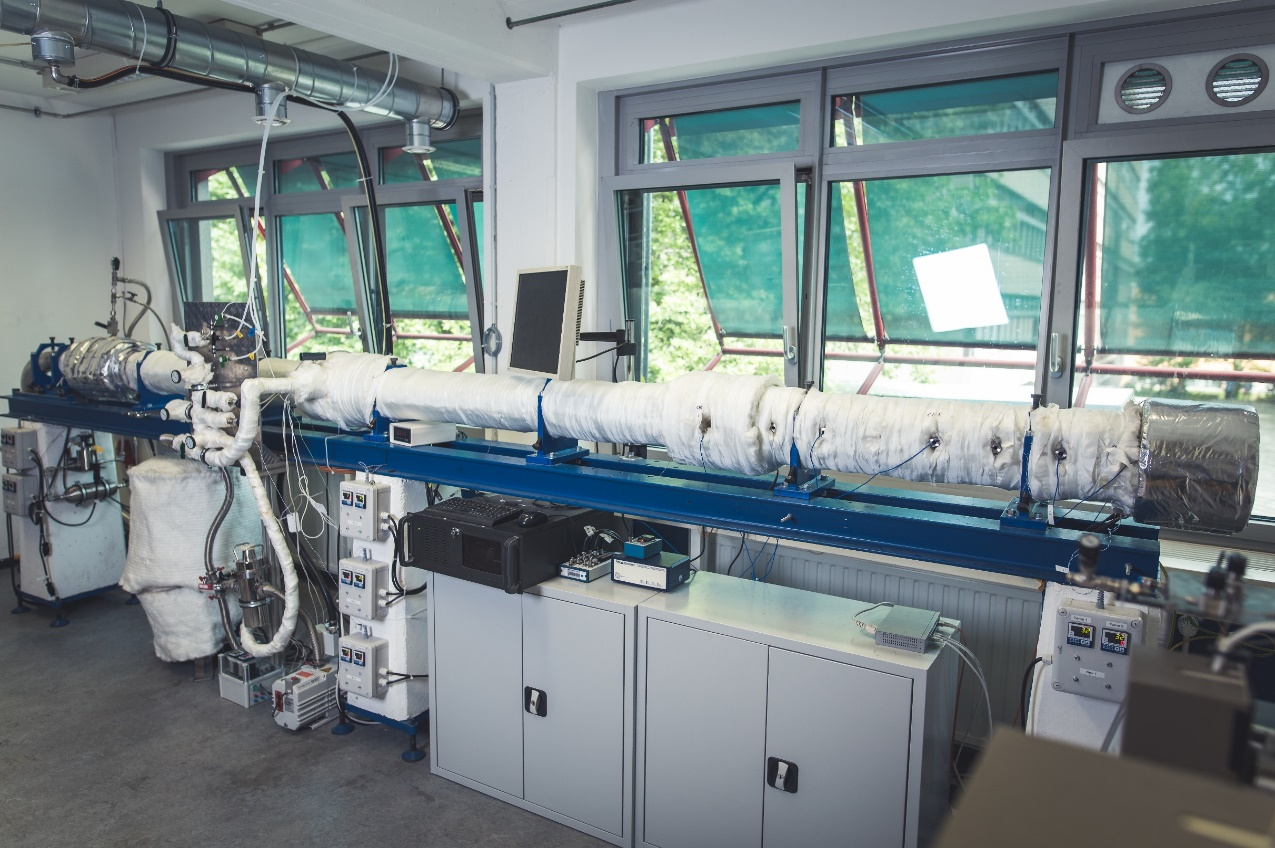
\includegraphics[width=0.9\columnwidth]{../figures/PCFC_ST.jpg}
			WOW!
			\columnbreak
			\begin{enumerate}
				\item Shock tubes are cool
				\item Ours is hot!
			\end{enumerate}	
		\end{multicols}
	\end{block}
	\vfill
\end{beamercolorbox}
\end{column}
\end{columns}

%back to left /right columns
	\begin{columns}
	\begin{column}{.48\textwidth}
		\begin{beamercolorbox}[center,wd=\textwidth]{postercolumn}
			\begin{block}{\LARGE Introduction}
				\begin{itemize}
					\item Intro
				\end{itemize}	
			\end{block}
			\vfill
			\begin{block}{\LARGE Something about experiments}
				\begin{enumerate}
					\item Point 1
					\item Point 2
				\end{enumerate}	
			\end{block}
			\vfill
		\end{beamercolorbox}
	\end{column}
	% end left column
	% ---------------------------------------------------------%
	% start right column
	\begin{column}{.48\textwidth}
		\begin{beamercolorbox}[center,wd=\textwidth]{postercolumn}
			\begin{block}{\LARGE Introduction}
				Test citation\cite{Fuller.2014}.	
			\end{block}
			\vfill
			\begin{block}{\LARGE REFERENCES}
				 \printbibliography
			\end{block}
		\end{beamercolorbox}
	\end{column}
\end{columns}
  \vskip2ex
\end{frame}
\end{document}


%%%%%%%%%%%%%%%%%%%%%%%%%%%%%%%%%%%%%%%%%%%%%%%%%%%%%%%%%%%%%%%%%%%%%%%%